


\chapter{Observations}
  \label{ch_rbsp}

\todo{You know what would be great for putting this numerical work in context? A nice, consistent survey that breaks down the occurrence rate of Pc4 pulsations by harmonic, etc. }

%Observations show that the poloidal mode is most excited in the second harmonic\cite{cummings_1969,hughes_1978,arthur_1981,singer_1982,takahashi_1984,engebretson_1988} even when there is a strong compressional component\cite{takahashi_1987,haerendel_1999,vaivads_2001,sibeck_2012}. 

\todo{The tools used in the present chapter --- SPEDAS and the SPICE kernel --- are publicly available. They run best with an IDL license, which is not, but they are functional using just the (free) IDL virtual machine. The code is wrapped up in a Git repository: \url{https://github.com/chizarlicious/RBSP} (maybe should make a GitHub organization to hold this code, to decouple it from my personal account?). }

% -----------------------------------------------------------------------------
% -----------------------------------------------------------------------------
% -----------------------------------------------------------------------------
\section{Sampling Bias and Event Selection}
  \label{sec_selection}

The present analysis makes use of all available Van Allen Probe data, which spans from October 2012 to August 2015. Between the two probes, that's just over 2000 days of observation. 

For the purposes of Pc4 pulsations, it's reasonable to consider the two probes to be independent observers. Nearly all Pc4 events occur near apogee ($L\gtrsim5$), at which point the two probes are several hours apart in MLT. Pc4 events are typically not large enough to be seen by both probes simultaneously, and not long enough in duration to be seen by two probes passing through the same region of space several hours apart. 

\todo{Quantify how often an event is seen by both probes? }

Electric and magnetic field waveforms are collected using the probes' \todo{$\cdots$} instrument. Values are cleaned up by averaging over the ten-second spin period. Three-dimensional electric field data is then obtained using the $\vec{E} \cdot \vec{B} = 0$ assumption. Notably, this assumption is taken only when the probe's spin plane is offset from the magnetic field by at least \SI{15}{\degree}. The rest of the data --- about half --- is discarded, which introduces a sampling bias against the flanks. 

A further bias is introduced by the probes' non-integer number of precessions around Earth. As of July 2014, apogee had precessed once around Earth\cite{dai_2015}. The present work considers roughly one and a half precessions; the nightside has been sampled at apogee twice as often as the dayside. 

The spatial distribution of usable data --- that is, data for which three-dimensional electric and magnetic fields are available --- is shown in \cref{fig_pos_all_sharp}. Bins are unitary in $L$ and in MLT. Event distribution in magnetic latitude is not shown; the Van Allen Probes are localized to within \about\SI{10}{\degree} of the equatorial plane. 

\todo{$L$ is italicized and MLT is not? That seems weird. }

\begin{figure}[!htb]
    \centering
    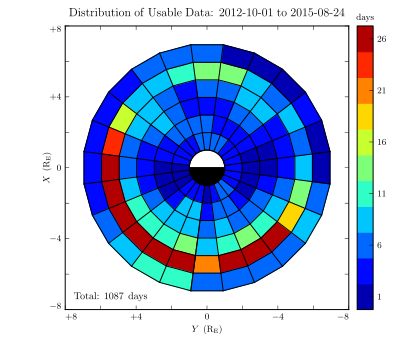
\includegraphics[width=\textwidth]{figures/pos_all_sharp.pdf}
    \caption[Distribution of Usable Van Allen Probe Data]{
      Three-dimensional electric field values are computed by assuming $\vec{E} \cdot \vec{B} = 0$. Data is discarded whenever the magnetic field falls within \SI{15}{\degree} of the spin plane, which introduces a bias against the flanks. Furthermore, the probes have completed one and a half precessions around Earth; the dayside has been sampled once at apogee, and the nightside twice. 
    }
    \label{fig_pos_all_sharp}
\end{figure}

Field measurements are transformed from GSE coordinates into the same dipole coordinates used in \cref{ch_model,ch_results}. The \z axis is parallel to the background magnetic field, which is estimated using a ten-minute running average of the magnetic field measurements. The \y axis is set parallel to $\zhat \times \vec{r}$, where \vec{r} is the probe's geocentric position vector. The \x axis is then defined per $\xhat \equiv \yhat \times \zhat$. This scheme guarantees that the axes are right-handed and pairwise orthogonal\cite{liu_2009}. 

The \about1000 days of usable data are considered half an hour at a time, which gives a frequency resolution of \about\SI{0.5}{\mHz} in the discrete Fourier transform. Spectra are computed for all six field components: \dft{B_x}, \dft{B_y}, \dft{B_z}, \dft{E_x}, \dft{E_y}, and \dft{E_z}. The background magnetic field is subtracted before transforming the magnetic field components, leaving only the perturbation along each axis\footnote{As in \cref{ch_model,ch_results}, $B_x$ refers not to the full magnetic field in the \x direction, but to the perturbation in the \x direction from the zeroth-order magnetic field.}. Each waveform is also shifted horizontally so that its mean over the thirty minute event is zero. 

Frequency-domain Poynting flux is computed from the electric and magnetic field transforms. A factor of $L^3$ compensates the compression of the flux tube, so that the resulting values are effective at the ionosphere. Poloidal and toroidal Poynting flux, respectively, are given by:
\begin{align}
  \dft{S_P} &\equiv -\frac{L^3}{\mz} \dft{E_y} \dft{B_x^*} &
  \dft{S_T} &\equiv  \frac{L^3}{\mz} \dft{E_x} \dft{B_y^*}
\end{align}

The poloidal and toroidal channels are independently checked for Pc4 waves. For each channel, a Gaussian profile is fit to the magnitude of the Poynting flux, $|\dft{S}\arg{\omega}|$. If the fit fails to converge, or if the peak of the Gaussian does not fall within \SI{5}{\mHz} of the peak value of \dft{S}, the event is discarded. Events are also discarded if their frequencies fall outside the Pc4 frequency range (\SIrange{7}{25}{\mHz}) or if their amplitudes fall below \SI{e-2}{\mW/\m\squared} (out of consideration for instrument sensitivity). 

Events are discarded if their parity is ambiguous. The electric field and the magnetic field must be coherent at a level of 0.9 or better (judged at the discrete Fourier transform point closest to the peak of the Gaussian fit). Any event within \SI{3}{\degree} of the magnetic equator is also not used; as discussed in \cref{ch_flrs}, in order to distinguish an odd mode from an even mode, it's necessary to know whether the observation is made north or south of the equator. 

\todo{How much time do the probes spend within \SI{3}{\degree} of the magnetic equator? }

A visual inspection of events shows that those with broad ``peaks'' in their spectra are typically not peaked at all --- they are noisy spectra with several spectral features grouped just closely enough to trick the fitting routine. A threshold is set at a FWHM of \SI{3}{\mHz} (equally, a standard deviation of \SI{1.27}{\mHz}). Any event with a Gaussian fit broader than that is discarded. 

Notably, events are not filtered on their phase --- that is, on the division of their energy between standing and traveling waves. This is the topic of \cref{sec_phase}. 

\todo{First and third harmonics can only be distinguished by guessing at the frequency. Chisham and Orr\cite{chisham_1991} argue that around \SI{7}{\RE}, frequency around \SI{10}{\mHz} precludes higher harmonics. Or maybe look at \cite{green_1985}? }

\todo{Are we biased in terms of \DST? What's the distribution look like for the good data and for the bad data? }

% -----------------------------------------------------------------------------
% -----------------------------------------------------------------------------
% -----------------------------------------------------------------------------
\section{Events by Mode}
  \label{sec_rate}

The filters described in \cref{sec_selection} yield 762 Pc4 events, the spatial distribution of which is shown in \cref{fig_rate_all_sharp}. In each bin, the event count is normalized to the amount of usable data, per \cref{fig_pos_all_sharp}. Bins shown in white contain zero events. The rate in the bottom corner is an overall mean, weighing each bin equally. 

\todo{Bins should be weighted by $L$. The small inner bins count too much right now, and are dragging down the average. }

\begin{figure}[!htb]
    \centering
    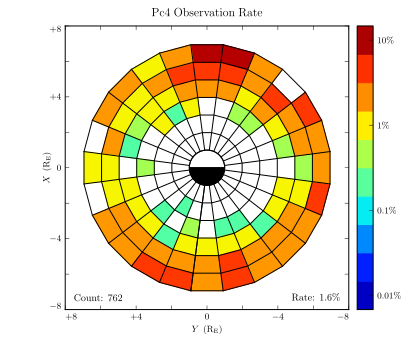
\includegraphics[width=\textwidth]{figures/rate_all_sharp.pdf}
    \caption[Observation Rate of Pc4 Events]{
      The above figure shows the spatial distribution of all 762 observed Pc4 events. Counts are normalized by the amount of usable data in each bin. The value in the bottom-right corner is the mean of the rate in each bin; it's an estimate of how often Pc4 events would be observed if the sampling were distributed uniformly in space. Events where the poloidal and toroidal channel trigger simultaneously (\about\SI{10}{\percent} of cases) are counted as only a single event. Bins shown in white contain zero events. 
    }
    \label{fig_rate_all_sharp}
\end{figure}

Consistent with previous work, Pc4 events peak on the dayside and are rarely observed at $L < 4$. Nearly \SI{30}{\percent} of the usable data shown in \cref{fig_pos_all_sharp} is located inside $L = 4$, yet that data accounts for only 16 of the 762 events. 

On the other hand, the present work runs contrary to Dai's 2015 result in terms of Pc4 event rates with respect to the plasmapause (not shown). His analysis found Pc4 pulsations to be comparably common inside and outside the plasmapause\cite{dai_2015}. In the present work, only 40 of the 762 events (\SI{5}{\percent}) fall inside the plasmasphere, despite the fact that \SI{40}{\percent} of the available data falls within the plasmasphere. The disparity is not likely due to a difference in sampling --- Dai's work, like the present work, uses data from the Van Allen Probes mission. Rather, the difference is likely due to disagreement in how the plasmapause is defined. Dai identifies the plasmapause by the maximum gradient in electron number density, while the present work takes an electron density of \SI{100}{\percc} to mark the plasmapause\footnote{Per ongoing work by Thaller. }. 

In \cref{fig_mode_all_sharp}, events are partitioned by parity and polarization, yielding 124 odd poloidal events, 214 even poloidal events, 415 odd toroidal events, and 83 even toroidal events --- a total of 836 events. The total is greater than 762 because in \about\SI{10}{\percent} of events, the poloidal and toroidal channels trigger independently. Such cases are marked as a single event in \cref{fig_rate_all_sharp}, but the toroidal and poloidal events are both shown in \cref{fig_mode_all_sharp}. 

Double-triggering can be taken as a vague proxy for event quality. When the channels both trigger independently, the two events almost always (71 of 74 events) exhibit the same parity. This suggests a poloidal wave with suffient power, and a sufficient narrow spectral peak, that it can still be seen after much of its energy has rotated to the toroidal mode. 

Odd double-triggering events are spread broadly in MLT. They rarely occur twice on the same day (23 events spread over 20 days), are observed at comparable rates regardless of \DST. 

Even-harmonic double-triggering events, on the other hand, are mostly seen near noon, and are significantly more common when $\DST < \SI{-30}{\nT}$. Even events are also more concentrated than odd ones. The 48 even-harmonic double-events are spread over 20 days, and 35 of them are spread over just 7 days. This clustering --- where the poloidal and toroidal channel both trigger for five to ten half-hour events in the same day --- is prevalent regardless of \DST. 

\begin{figure}[!htb]
    \centering
    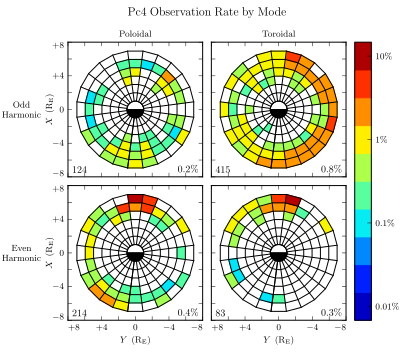
\includegraphics[width=\textwidth]{figures/mode_all_sharp.pdf}
    \caption[Observation Rate of Pc4 Events by Mode]{
      The above figure shows the spatial distribution for the same 762 events shown in \cref{fig_rate_all_sharp}, partitioned by polarization and parity. The selection criteria described in \cref{sec_selection} ensure that both properties are known for all events. Event counts are normalized by the time spent by the amount of usable data in each bin. Counts shown in the bottom-left corners do not sum to 762 because some events trigger on both the poloidal channel and the toroidal channel. Bins shown in white contain zero events. 
    }
    \label{fig_mode_all_sharp}
\end{figure}

The distribution of even poloidal events in \cref{fig_mode_all_sharp} is consistent with that reported by Dai\cite{dai_2015}: the observation rate is peaked at noon, and smeared across the dusk side. Notably, Dai's work focused on even poloidal waves. While he did not explicitly remove odd events from his sample, he did introduce a threshold in the magnetic field. This threshold is preferrentially satisfied by even waves (which have a magnetic field antinode near the equator) compared to odd waves (which have a magnetic field node). Dai characterized the parity of only a quarter of his events; among those, he found even harmonics to outnumber odd harmonics ten-to-one. 

In fact --- to the degree that they can be straightforwardly compared --- the distributions in \cref{fig_mode_all_sharp} also show agreement with work by Anderson (using AMPTE/CCE\cite{anderson_1990}), Kokubun (using ATS6\cite{kokubun_1989}), Liu (using THEMIS\cite{liu_2009}), and Motoba (using GOES\cite{motoba_2015}). Toroidal events dominate overall, and are primarily seen on the dawn side. Poloidal events are spread broadly in MLT, with a peak near noon and distinctive odd harmonics in the early morning. 

Crucially, the present work can offer insight into how previous results fit together. Unlike events considered in previous works, those shown in \cref{fig_mode_all_sharp} have all been categorized in terms of both polarization and parity. And, perhaps more importantly, the selection process has not introduced a bias with respect to polarization or parity (at least not an obvious one). 

Not only does \cref{fig_mode_all_sharp} show that toroidal events outnumber poloidal events, but it also shows that toroidal events are predominantly odd harmonics --- as opposed to the primarily-even poloidal events. This may suggest that odd poloidal waves are more likely than even ones to be driven at low modenumber (allowing a prompt rotation of that energy to the toroidal mode). One might expect low-\azm poloidal modes to be driven by a sudden increase in the solar wind dynamic pressure, for instance. The relative scarcity of odd poloidal observations on the dayside may indicate a short-lived source. At low \azm, energy rotates to the toroidal mode on the order of a wave period; without an ongoing source, there will be no poloidal wave to observe. 


\todo{Also, even waves are less likely to produce ground signatures\cite{takahashi_1992}, perhaps because they are more likely to be at high modenumber? }



\todo{People have talked about this. Is there a conventional explanation for dawn-dusk asymmetry? }

Even poloidal modes and even toroidal modes exhibit similar distributions in space: both are peaked at noon and smeared across the dusk flank, with little activity on the dawn side. This is consistent with the idea that the even poloidal mode is a significant source for the even toroidal mode. 

\todo{What else do we want to say here? Or does the rest of the commentary belong in the later sections? Note that plots in future sections are lower resolution, to make sure that the number of bins remains much smaller than the number of events. }

%Dai\cite{dai_2015} used RBSP to look at poloidal Pc4 events, with a bias in favor of the second harmonic --- 890 events. Events are most common near noon, but are spread across the day and dusk side, with a few stragglers at midnight. 

%Anderson\cite{anderson_1990} used AMPTE/CCE (mostly $L>7$, near the equator) to look at Pc4 events --- 7000 hours. Limited commentary on parity. Toroidal modes were found to outnumber poloidal modes three-to-one. ``Harmonic toroidal resonances'' are spread 0600 to 1600. ``Fundamental toroidal resonances'' (which are not mutually exclusive with harmonic ones!) appear everywhere but dusk. 

%Liu\cite{liu_2009} used THEMIS (equatorial orbit, $L$ out to \about10) to look at both poloidal and toroidal modes --- 9805 one-minute Pc4 events (?). No commentary on parity. Poloidal events are most common at noon (with another peak post-midnight) and strongest on the dusk side. Toroidal events are most common from pre-dawn to pre-noon and strongest pre-midnight and post-dawn. 

%Kokubun\cite{kokubun_1989} used ATS6 (synchronous orbit) --- \about150 events. No commentary on harmonic. Toroidal events dominate in the dawn sector. Poloidal events are spread across all MLT, with a peak in the early afternoon and Pgs in the early morning. 

%Motoba\cite{motoba_2015} used GOES13 and GOES15 (geosynchronous) to look specifically at Pgs --- 105 events. Seen from midnight to noon, with a strong peak before dawn, 0300 or so. 

%\todo{Even poloidal events and even toroidal events are distributed similarly, which is good to see, since even poloidal events give rise to even toroidal events. The relationship is less clear for odd events, though odd poloidal modes and odd toroidal modes are both least common at dusk. }

%\todo{Odd toroidal events are by far the most commonly observed. Oddly, even poloidal events are the least common. }

%\todo{Even modes are less likely to be observed on the ground? \cite{takahashi_1992} }

% -----------------------------------------------------------------------------
% -----------------------------------------------------------------------------
% -----------------------------------------------------------------------------
\section{Events by Amplitude}
  \label{sec_amp}

One might reasonable be concerned that the spatial distributions presented in \cref{fig_mode_all_sharp} are dominated by these small events, while Pc4 events large enough to be noteworthy follow a different distribution entirely. The goal of the present section is to address that concern. 

\begin{figure}[!htb]
    \centering
    \includegraphics[width=\textwidth]{figures/amp.pdf}
    \caption[Amplitude Distribution of Pc4 Events by Mode]{
      \todo{$\cdots$}
    }
    \label{fig_amp}
\end{figure}

The distribution of event magnitudes is presented in \cref{fig_amp}, graded based on the peak of the Gaussian fit of each event's Poynting flux, $|\dft{S}\arg{\omega}|$. Mean and median values are listed for each mode. Most events are small, with Poynting flux well below \SI{0.1}{\mW/\m\squared} when mapped to the ionosphere. Only a handful of events --- 3 out of 762 --- exceed \SI{1}{\mW/\m\squared}, typically taken to be the threshold at which visible auroral arcs form. One such event is shown in \cref{fig_sample_event_strong}. 

\todo{Say something about this event? Not really clear what purpose is served by this example, actually. As a matter of curiosity, the apparent wave activity in the toroidal channel did not pass the event selection trigger because the electric and magnetic waveforms are not coherent. }

\begin{figure}[!htb]
    \centering
    \includegraphics[width=\textwidth]{figures/sample_event_strong.pdf}
    \caption[Waveforms and Spectra for a Strong Pc4 Event]{
      \todo{$\cdots$}
    }
    \label{fig_sample_event_strong}
\end{figure}

\todo{The distribution of even poloidal events is flatter in amplitude than the rest. As the amplitude cutoff increases, so does the proportion of even events. }

\todo{The distribution of events by mode is reproduced in \cref{fig_mode_amp} using several different amplitude cutoffs. The qualitative distribution of events does not change. }

\begin{figure}[!htb]
    \centering
    \includegraphics[width=\textwidth]{figures/mode_amp.pdf}
    \caption[Observation Rate of Pc4 Events by Mode and Amplitude]{
      \todo{$\cdots$}
    }
    \label{fig_mode_amp}
\end{figure}


% -----------------------------------------------------------------------------
% -----------------------------------------------------------------------------
% -----------------------------------------------------------------------------
\section{Events by Frequency}
  \label{sec_f}

\todo{(Odd) toroidal events exhibit a much stronger peak in frequency than poloidal events. This is consistent with the fact that toroidal waves align closely with the local eigenfrequency, while poloidal modes are more smeared in $L$, as discussed in \cref{sec_day}. Van Allen Probe observations are mostly concentrated over a small range in $L$ near apogee. }

\todo{Maybe put the Gaussian fit back on top of these distributions? The distributions are not particularly Gaussian, but it gives a quantitative estimate of the spread. }

\begin{figure}[!htb]
    \centering
    \includegraphics[width=\textwidth]{figures/f.pdf}
    \caption[Frequency Distribution of Pc4 Events by Mode]{
      \todo{$\cdots$}
    }
    \label{fig_f}
\end{figure}


\begin{figure}[!htb]
    \centering
    \includegraphics[width=\textwidth]{figures/mode_f.pdf}
    \caption[Observation Rate of Pc4 Events by Mode and Frequency]{
      \todo{$\cdots$}
    }
    \label{fig_mode_f}
\end{figure}


% -----------------------------------------------------------------------------
% -----------------------------------------------------------------------------
% -----------------------------------------------------------------------------
\section{Events by Phase}
  \label{sec_phase}

The phase of a wave --- that is, the phase offset between a wave's electric and magnetic fields --- indicates how its energy is partitioned between the standing and traveling wave modes. An ideal standing wave has a phase of $\pm$\SI{90}{\degree}, and thus its Poynting flux is completely imaginary. A traveling wave, on the other hand, has electric and magnetic fields in phase (or in antiphase), and is associated with a net movement of energy, usually toward the ionosphere. 

Wave phase is a topic of significant interest, since it allows an estimate to be made of the wave's lifetime. And, because phase can only be determined using simultaneous electric and magnetic field measurements, it has only recently become observable. 

\todo{Do people really care about phase, or is it just John? }

The energy per unit volume, and the rate at which energy is carried out of that volume by Poynting flux, are respectively given by:
\begin{align}
  \label{def_phase}
  U &= \frac{R^3}{2\mz} B^2 &
  \ddt U &= \frac{R^2}{\mz} E B \cos\varphi
\end{align}

Where $B$, $E$, and $R$ are the characteristic magnetic field magnitude, electric field magnitude, and length scale. The phase, $\varphi \equiv \arctan\frac{ \imag\dft{S} }{ \real\dft{S} }$, enters because only real Poynting flux carries energy. 

The ratio of the two quantities in \cref{def_phase} gives a characteristic timescale over which energy leaves the system
\begin{align}
  \label{def_tau}
  \tau &\equiv \frac{BR}{2 E \cos\varphi}
\end{align}

In the present case, magnetic fields are on the order of \SI{1}{\nT} and electric fields are on the order of \SI{1}{\mV/\m}. A reasonable scale length might be \SI{e4}{\km}, the distance traversed by the probe over the course of a half-hour event (notably, back-to-back events are unusual). 

At a phase of \SI{80}{\degree}, this timescale is comparable to a Pc4 wave period. At \SI{135}{\degree}, where energy is divided evenly between the standing and traveling wave, the timescale is only 7 seconds. A wave with a phase so far from \SI{90}{\degree} would quickly vanish unless it were constantly being replenished. 

An example of just such an event is shown in \cref{fig_sample_event_phase}.  The left column shows electric and magnetic field waveforms in blue and red respectively. The right shows the corresponding spectra: imaginary Poynting flux in magenta (corrresponding to the strength of the standing wave) and real Poynting flux in green (for the traveling wave). The black line is a Gaussian fit to the magnitude of the Poynting flux. 

The poloidal channel shows a mostly-standing wave, with a phase of \SI{79}{\degree}. The coherent activity in the compressional magnetic field implies a low azimuthal modenumber, and thus a fast rotation of energy from the poloidal mode to the toroidal mode. It's likely the rotation of energy from the poloidal mode is the only thing keeping the toroidal wave going; its phase is \SI{130}{\degree}, so its energy should be carried away by Poynting flux quickly compared to the oscillation of the standing wave. 

\begin{figure}[!htb]
    \centering
    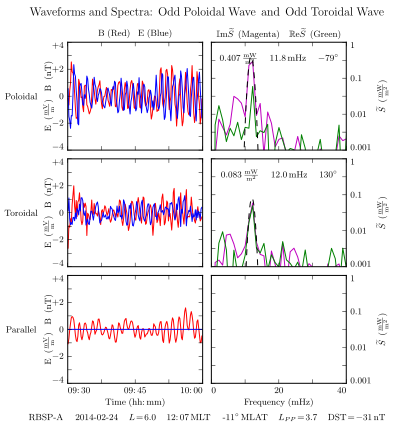
\includegraphics[width=\textwidth]{figures/sample_event_phase.pdf}
    \caption[Waveforms and Spectra for a Pc4 Event]{
      The above is a double event, where the poloidal and toroidal channels have been independently selected as events. The poloidal channel shows a wave with most of its energy in the standing wave (phase of \SI{79}{\degree}). The toroidal mode has a significant traveling component (phase of \SI{130}{\degree}). The compressional activity implies a low modenumber, which would cause energy to rotate quickly from the poloidal mode to the toroidal mode --- evidently at a sufficient rate to replenish the losses due to the traveling mode's real Poynting flux. 
    }
    \label{fig_sample_event_phase}
\end{figure}

The selection process described in \cref{sec_selection} does not explicitly consider phase. However, the discrete Fourier transform is performed over a half-hour time span. An event with a comparatively short lifetime would be unlikely to register. It's unsurprising to see the events in \cref{fig_phase}tightly clustered near \SI{90}{\degree}. 

\begin{figure}[!htb]
    \centering
    \includegraphics[width=\textwidth]{figures/phase.pdf}
    \caption[Phase Distribution of Pc4 Events by Mode]{
      \todo{$\cdots$}
    }
    \label{fig_phase}
\end{figure}

It's further notable in \cref{fig_phase} that the odd events are more spread out in phase than the even events. Near the equator, odd modes have an electric field antinode and a magnetic field node; per \cref{def_tau}, an odd mode's lifetime should be longer than that of an even mode with the same phase. 

\todo{The spatial distribution of Pc4 events doesn't seem to depend much on phase, as shown in \cref{fig_mode_phase}. }

\begin{figure}[!htb]
    \centering
    \includegraphics[width=\textwidth]{figures/mode_phase.pdf}
    \caption[Observation Rate of Pc4 Events by Mode and Phase]{
      \todo{$\cdots$}
    }
    \label{fig_mode_phase}
\end{figure}

% -----------------------------------------------------------------------------
% -----------------------------------------------------------------------------
% -----------------------------------------------------------------------------
%\section{Poloidal Pc4 Events by Compressional Coupling}

%\todo{Low-\azm poloidal Pc4 events are coupled to the compressional mode, while high-\azm ones are not. }

%\todo{The value of $\dft{B_z}/\dft{B_x} = 0.2$ comes from Dai\cite{dai_2015}. Can we match this up to an \azm value? Sounds like a job for Tuna! }

%\begin{figure}[!htb]
%    \centering
%    \includegraphics[width=\textwidth]{figures/azm_rate_all.pdf}
%    \caption[Poloidal Pc4 Rate by Compressional Coupling]{
%      \todo{Odd poloidal Pc4 events have a peak pre-noon and another peak near midnight. The pre-noon peak seems to be composed of high-\azm events, and the midnight peak seems to be low-\azm events. Low-\azm even poloidal events are spread broadly across the dusk side, while high-\azm even events are peaked strongly on the dayside --- consistent with Dai's results\cite{dai_2015}. }
%    }
%    \label{fig_azm_rate_all}
%\end{figure}


% -----------------------------------------------------------------------------
% -----------------------------------------------------------------------------
% -----------------------------------------------------------------------------
\section{Discussion}

\todo{$\cdots$}



%\todo{Collections of events at a single ground observatory (near \SI{66}{\degree}) over significant periods of time: }

%Brekke\cite{brekke_1987} looked at 523 giant pulsation events recorded at Troms{\o}, Norway, from 1929 to 1985. This spanned several solar cycles. 

%Rolf\cite{rolf_1931} collected 28 events between 1921 and 1930 at Abisko. 

%Sucksdorf\cite{sucksdorff_1939} got 150 events between 1914 and 1938 in Sodankyl{\"a}. 

%Harang\cite{harang_1941}. 97 events from 1929 to 1941. Also Troms{\o}. Note that this may have been limited by the war! 

%This comes out to something like ... events over ... years. That's about ... giant pulsations per year, observed on the ground. 

%\todo{Collections of events at an array of ground observatories: }

%Chisham and Orr\cite{chisham_1991} found 34 events from 1984 to 1987 using the EISCAT magnetometer array in scandanavia. About \SI{5}{\degree} in MLT, decent coverage from \SIrange{63}{67}{\degree} mlat. This coincides with a solar minimum. 

%Motoba, in 2015, recorded 105 giant pulsation events. The observations were carried out by a number of ground magnetometers spanning $\sim \SI{90}{\degree}$ in local time and ranging roughly \SIrange{60}{70}{\degree} magnetic latitude\cite{motoba_2015}. This was mostly during a period of low solar activity, so we expect a high count. 

%\todo{Estimate of the size of an event's footprint:}

%Velkamp\cite{veldkamp_1960} looked at a single large event and showed that, at best, it was visible over a span of \SI{5}{\degree} in magnetic latitude. 

%This is seemingly consistent with the 29 February 2012 event discussed in detail by Motoba\cite{motoba_2015} --- Motoba shows some data, but doesn't discuss this aspect in detail. 

%Takahashi\cite{takahashi_2011} computes a FWHM of about 1 in L, or \SI{2}{\degree} magnetic latitude. 

%\todo{Tying that in to RBSP observations? }

%Note that it's a bit tricky to compare ground observations to in situ observations. Large-\azm events won't make it through the ionosphere. 

%There should be no bias with respect to MLT between a ground magnetometer and RBSP. Dai's analysis was specifically chosen to take advantage of the fact that RBSP's orbit had precessed all the way around the Earth. No preferred direction. And mlat shouldn't cause issues... these are FLRs, after all. 

%How strong does an event need to be on the ground, or in the sky, to count as a giant pulsation? Motoba 2015\cite{motoba_2015} has an event which tops out on the order of \SI{10}{\nT} on the ground. It's more like \SI{5}{\mV/\m} in situ. Takahashi\cite{takahashi_2011} has similar values. 

%If peak Pg observations are at $\SI{66}{\degree}$ mlat, that corresponds to $L = 6$. Then let's suppose that peak Pg viewing is $\SI{5}{\degree}$ wide --- estimating from the work of Velkamp and Motoba. That means RBSP should see lots of Pgs when it's between $L = 5.2$ andn $L = 7.1$. Well, \SI{7.1}{\RE} is outside its apogee, but the probes spend a fair amount of time outside $L = 5.2$, since they are moving pretty slowly at that point. 

%Giant pulsations have been shown to be more numerous in times of low solar activity. That was the whole point of Brekke's seminal 1987 paper, and it's consistent with what we show in \cref{ch_results}. The RBSP observations occur during peak solar times, though it's an anemic solar peak\cite{pesnell_2016}. 

%\todo{How much time does RBSP spend outside of $L = 5.2$ (for a range of \SI{5}{\degree})? How about $L = 5.6$ to $L = 6.5$ (for FWHM of \SI{2}{\degree}? }

%Each RBSP probe spends about \SI{30}{\percent} of its orbit between $L = 5.6$ and $L = 6.5$. 

%RBSP-A and RBSP-B count as two observers. In one $\sim 5$ cases out of hundreds do they simultaneously observe a poloidal Pc4 event (although, most notably for the 2012 event which \cite{dai_2013} considers in detail), both probes do fly through the same apparent event several hours apart from one another. 

%The duration of Dai's survey is October 2012 to June 2014. Scaled by 2 probes, each of which is present in the peak Pg lshells 30\% of the time, that comes out to almost exactly one year. 

%\todo{How many fundamental mode poloidal events do we see? How many could pass for giant pulsations? How many should we expect to see? }

%\todo{How weird is it for a fundamental mode poloidal Pc4 to be monochromatic? }

%\todo{How weird is it for a fundamental mode poloidal Pc4 to be stronger than \SI{5}{\mV/\m} at the equator? }






